\documentclass{standalone}
\usepackage{tikz}
\author{D.A.Pelasgus}

\begin{document}
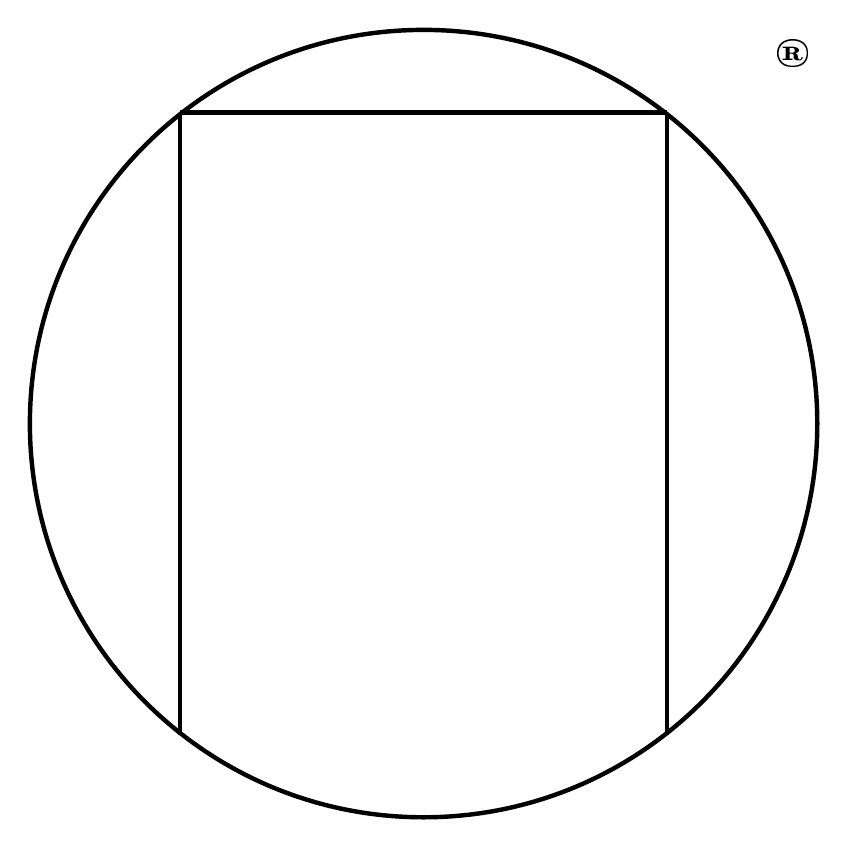
\begin{tikzpicture}

    % Define the circle with center at (0,0) and radius 100 units
    \draw[ultra thick, black] (0,0) circle[radius=5cm];

    % Horizontal line of Pi (centered, width based on golden ratio)
    \draw[ultra thick, black] (-3.09, 3.95) -- (3.09, 3.95);
    
    % Left vertical line of Pi (touching top and bottom inside the circle)
    \draw[ultra thick, black] (-3.09, 3.95) -- (-3.09, -3.95);
    
    % Right vertical line of Pi (touching top and bottom inside the circle)
    \draw[ultra thick, black] (3.09, 3.95) -- (3.09, -3.95);

    % Add a registered trademark symbol in the top right corner of the viewbox
    \node[black] at (4.7, 4.7) {\textbf{\textregistered}};
    
\end{tikzpicture}
\end{document}
